% !TeX program = XeLaTeX
% !TeX root=./main.tex
% Edit by:XAjzh
\setlength{\abovedisplayskip}{5pt}
\setlength{\belowdisplayskip}{5pt}

\chapter{多维随机变量及其分布}\label{cha:3}
在有些随机现象中, 对每个样本点 $\omega$ 只用一个随机变量去描述是不够的, 
譬如要研究儿童的生长发育情况, 仅研究儿童的身高 $X(\omega)$ 或仅研究其体重 $Y(\omega)$都是片面的, 
有必要把 $X(\omega)$ 和 $Y(\omega)$ 作为一个整体来考虑, 讨论它们总体变化的统计规律性, 
进一步可以讨论 $X(\omega)$ 与 $Y(\omega)$ 之间的关系, 在有些随机现象中, 甚至要同时研究二个以上随机变量. 

如何来研究多维随机变量的统计规律性呢, 仿一维随机变量, 我们先研究联合分布函数, 
然后研究离散随机变量的联合分布列、连续随机变量的联合密度函数. 

\section{多维随机变量及其联合分布}\label{sec:3.1}

\subsection{多维随机变量}\label{ssec:3.1.1}
下面我们先给出 $n$ 维随机变量的定义. 
\begin{definition}{随机变量}{3.1.1}
	如果 $X_1(\omega),X_2(\omega),\ldots,X_n(\omega)$ 是定义在同一
	样本空间 $\Omega=\left\{\omega\right\}$ 上的 $n$ 个随机变量, 则称
	\[
	X(\omega)=(X_1(\omega),X_2(\omega),\ldots,X_n(\omega))
	\]
	为 $n$ 维(或 $n$ 元)\textbf{随机变量}\index{S!随机变量}或\textbf{随机向量}\index{S!随机向量}. 
\end{definition}
注意, 多维随机变量的关键是定义在同一样本空间上, 对于不同样本空间上的两个随机变量, 我们只能在
乘积空间 $\Omega_1\times \Omega_2=\left\{(\omega_1,\omega_2);\omega_1 \in \Omega_1,\omega_2 \in \Omega_2 \right\}$ 上讨论, 
 这要用到更多的工具, 本章将不涉及这类问题. 
      
 在实际问题中, 多维随机变量的情况是经常会遇到的臂如
  \begin{itemize}
  	\item 在研究四岁至六岁儿童的生长发育情况时, 我们感兴趣于每个儿童(样本点 $\omega$ )的身高 $X_1(\omega)$ 
  	和体重 $X_2(\omega)$ . 这里 $(X_1(\omega),X_2(\omega))$是一个二维随机变量. 
  	\item 在研究每个家庭的支出情况时, 我们感兴趣于每个家庭(样本点 $\omega$ )的衣食住行四个方面, 
  	若用 $X_1(\omega),X_2(\omega),X_3(\omega),X_4(\omega)$ 分别表示衣食住行的花费占其家庭总收人的百分比, 
  	则 $X_1(\omega),X_2(\omega),X_3(\omega),X_4(\omega)$ 就是一个四维随机变量. 
  \end{itemize}

  \subsection{联合分布函数}\label{ssec:3.1.2}
  \begin{definition}{联合分布函数}{3.1.2}
  	对任意的 $n$ 个实数 $x_1,x_2,\ldots,x_n ,$ 则 $n$ 个事件 $\{X_1\leq x_1\},\{X_2 \leq x_2\},\ldots,\{X_n\leq x_n\}$ 同时发生的概率
    \begin{equation}
    	F\left(x_{1}, x_{2}, \cdots, x_{n}\right)=P\left(X_{1} \leq x_{1}, X_{2} \leq x_{2}, \ldots, X_{n} \leq x_{n}\right)\label{eq:3.1.1}
    \end{equation}
	称为 $n$ 维随机变量 $(X_1,X_2,\ldots,X_n)$ 的\textbf{联合分布函数}\index{L!联合分布函数}. 
  \end{definition}
   本章主要研究二维随机变量, 二维以上的情况可类似进行. 

   在二维随机变量 $(X,Y)$ 场合, 联合分布函数 $F(x,y)=P(X\leq x,Y\leq y)$ 是事件 $\{X\leq x\}$ 与 $\{Y \leq y\}$ 同时发生(交)的概率. 
   如果将二维随机变量 $(X,Y)$ 看成是平面上随机点的坐标, 那么联合分布函数 $F(x,y)$ 在 $(x,y)$ 处的函数值就是随机点 $(X, Y)$ 落在
   以 $(x,y)$ 为右上角的无穷矩形内的概率, 见图~\ref{fig:3.1.1} .
   \begin{figure}[htbp]
   	\centering
   	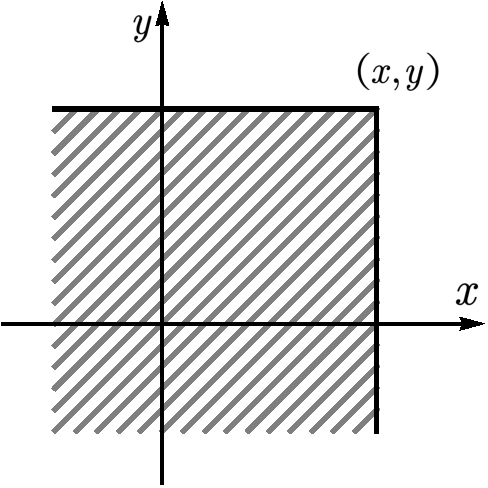
\includegraphics[width=0.4\textwidth]{fig3-1-1.pdf}
   	\caption{联合分布函数示意图}\label{fig:3.1.1}
   \end{figure}
   \begin{theorem}{}{3.1.1}
   	任一二维联合分布函数 $F(x,y)$ 必具有如下四条基本性质: 
    \begin{enumerate}
    	\item \textbf{单调性}\quad $F(x,y)$ 分别对 $x$ 或 $y$ 是单调不减的,即
    	\begin{itemize}
    		\item 当 $x_1<x_2$ 时, 有 $F(x_1,y)\leq F(x_2,y)$.
    		\item 当 $y_1<y_2$ 时, 有 $F(x,y_1)\leq F(x,y_2)$. 
    	\end{itemize}
    	\item \textbf{有界性}\quad 对任意的 $x$ 和 $y$, 有 $0\leq F(x,y) \leq 1$, 且
    	\begin{align*}
    		&F(-\infty,y)=\lim_{x\to -\infty}F(x,y)=0,	&\hspace*{3cm} \\
    		&F(x,-\infty)=\lim_{y\to -\infty}F(x,y)=0,	&\\
    		&F(+\infty,+\infty)=\lim_{x,y\to +\infty}(x,y)=1.&
    	\end{align*}
    	\item \textbf{右连续性}\quad  对每个变量都是右连续的,即
    		\begin{align*} 
    			F(x+0, y) &=F(x, y), &\hspace*{3cm} \\ 
    			F(x, y+0) &=F(x, y). &
    		\end{align*}
    	\item \textbf{非负性}\quad 对任意的 $a<b,c<d$ 有
    		\begin{equation*}
    		 	P(a<X \leq b, c<Y \leq d)= F(b, d)-F(a, d)-F(b, c)+ F(a, c) \geq 0 .
    		\end{equation*}
    \end{enumerate}
   \end{theorem}
   \begin{proof}
    	\begin{enumerate}
    		\item  因为当 $x_1<x_2$ 时, 有 $\{X_1\leq x_1\} \subset \{X_2 \leq x_2\}$, 所以对任意给定的 $y$ 有
    		\[
    			\left\{X \leq x_{1}, Y \leq y\right\} \subseteq \{ X \leq x_{2}, Y \leq y \},
    		\]
    		由此可得
    		\[
    			F\left(x_{1}, y\right)=P\left(X \leq x_{1}, Y \leq y\right) \leq 
    			P\left(X \leq x_{2}, Y \leq y\right)=F\left(x_{2}, y\right),
    		\]
    		即 $F(x,y)$ 关于 $x$ 是单调不减的, 同理可证 $F(x,y)$ 关于 $y$ 是单调不减的.
    		\item 由概率的性质可知 $0\leq F(x,y) \leq 1$. 又因为对任意的正整数 $n$ 有
    		\begin{align*}
    			&\lim_{x\to -\infty}\{X\leq x\}=\lim_{n\to +\infty}\bigcap_{m=1}^n \{X\leq -m\}=\varnothing,	\\
    			&\lim_{x\to +\infty}\{X\leq x\}=\lim_{n\to +\infty}\bigcup_{m=1}^n\{X\leq m\}=\Omega,
    		\end{align*}
    		对 $Y \leq y$ 也类似可得. 再由概率的连续性, 就可得
    		\[
    		 	F(-\infty, y)=F(x,-\infty)=0; \quad F(+\infty,+\infty)=1.
    		\]
    		\item 固定 $y$, 仿一维分布函数右连续的证明, 就可得知 $F(x, y)$ 关于 $x$ 是右连续的. 同样固定 $x$ 可
    		证得 $F(x,y)$ 关于 $y$ 是右连续的.
        	\item 只需证
        	\[
        	 	P(a<X \leq b, c<Y \leq d)=F(b, d)-F(a, d)-F(b, c)+F(a, c).
        	\]
        	为此记 ( 见图~\ref{fig:3.1.2} )
        	\[
        	 	A=\{X \leqslant a\}, \quad B=\{ X \leqslant b \}, \quad C=\{Y \leqslant c\}, \quad D=\{Y \leqslant d\},
        	\]
        	考虑到
        	\[
        	 	\{ a<X \leqslant b \}=B-A=B \cap \overline{A}, \quad\{c<Y \leqslant d\}=D-C=D \cap \overline{C},
        	\]
        	且 $A \subset B, C\subset D,$ 由此可得
        	\begin{align*}
        		 0 & \leqslant P(a<X \leqslant b, c<Y \leqslant d) \\ 
        		 &=P(B \cap \overline{A} \cap D \cap \overline{C}) \\ 
        		 &=P(B D-(A \cup C)) \\ 
        		 &=P(B D)-P(A B D \cup B C D) \\ 
        		 &=P(B D)-P(A D \cup B C) \\ 
        		 &=P(B D)-P(A D)-P(B C)+P(A B C D) \\ 
        		 &=P(B D)-P(A D)-P(B C)+P(A C ) \\ 
        		 &=P(B D)-P(A D)-P(B C)+P(A B C D) \\ 
        		 &=F(b, d)-F(a, d)-F(b, c)+F(a, c). 
        	\end{align*}
    	\end{enumerate}
    \end{proof}
   \begin{figure}[htbp]
   	\centering
   	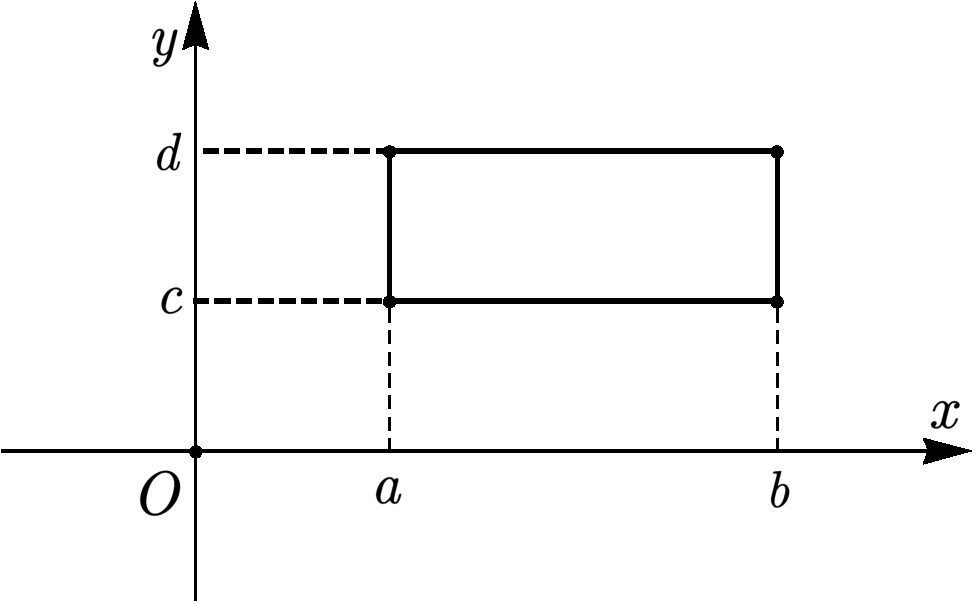
\includegraphics[width=0.4\textwidth]{fig3-1-2.pdf}
   	\caption{二维随机变量 $(X,Y)$ 落在矩形中的情况}\label{fig:3.1.2}
   \end{figure}
   还可证明,具有上述四条性质的二元函数 $F(x,y)$ 一定是某个二维随机变量的分布函数.

   任一二维分布函数 $F(x,y)$ 必具有上述四条性质, 其中性质 \textit{4} 是二维场合特有的, 也是合理的. 但性质 \textit{4} 不能
   由前三条性质推出, 必须单独列出, 且仅满足前三条性质是不够的, 因为存在这样的二元函数 $G(x,y)$ 满足
   以上性质 \textit{1,2,3}, 但它不满足性质 \textit{4}, 见下面例子.

   \begin{example}\label{exam:3.1.1}
   	二元函数
   	\[
   	 	G(x,y)=\begin{cases}
   	 		0,	& x+y<0;\\
   	 		1,	& x+y\geq 0 \\
   	 	\end{cases}
   	\]
   	满足二维分布函数的性质 \textit{1,2,3}, 但它不满足性质 \textit{4}.

    这从 $G(x,y)$ 的定义可看出: 若用 $x+y=0$ 将平面 $xOy$ 一分为二, 则
 
    $G(x,y)$ 在右上半平面 $(x+y\geq 0)$ 取值为1,
   
    $G(x,y)$ 在左下半平面 $(x+y\geq 0)$ 取值为0,

    $G(x,y)$ 具有非降性、有界性和右连续性, 但在正方形区域 $\{(x,y);-1\leq x\leq 1,-1\leq y\leq 1\}$的四个顶点上, 右上
    三个顶点位于右上半闭平面, 只有左下顶点 $(-1,-1)$ 位于左下半开平面, 故有
    \[
     	G(1,1)-G(1,-1)-G(-1,1)+G(-1,-1)=1-1-1+0=-1<0,
    \]
	所以 $G(x,y)$ 不满足性质 \textit{4}, 故 $G(x,y)$ 不能成为某二维随机变量的分布函数.
   \end{example}

   \subsection{联合分布列}\label{ssec:3.1.3}

   \begin{definition}{联合分布列}{3.1.3}
		如果二维随机变量 $(X,Y)$ 只取有限个或可列个数对 $(x_i,y_j)$, 则称 $(X,Y)$ 为二维离散随机变量, 称
    \begin{equation}\label{eq:3.1.2}
     	p_{i j}=P\left(X=x_{i}, Y=y_{j}\right), \quad i, j=1,2, \ldots
    \end{equation}
   	为 $(X,Y)$ 的\textbf{联合分布列}\index{L!联合分布列}, 也可如下用表格形式记联合分布列.
   \end{definition}
   \begin{center}
   		\begin{tabular}{cccccc}
   		\toprule
   		 & \multicolumn{5}{c}{$Y$} \\
   		 \cmidrule{2-6} 
   		 $X$	&	$y_1$&	$y_2$&	\ldots&	$y_j$& \ldots	\\
   		 \midrule 
   		 $x_1$& $p_{11}$ & $p_{12}$ & \ldots & $p_{1j}$ & \ldots \\
   		 \midrule 
   		 $x_2$& $p_{21}$ & $p_{22}$ & \ldots & $p_{2j}$ & \ldots \\
   		 \midrule 
   		 $\vdots$& $\vdots$ & $\vdots$ & $\ddots$ & $\vdots$ & $\ddots$ \\
   		 \midrule 
   		$x_i$ & $p_{i1}$ & $p_{i2}$ & \ldots & $p_{ij}$  & \ldots \\
   		\midrule 
   		 $\vdots$& $\vdots$ & $\vdots$ & $\ddots$ & $\vdots$ & $\ddots$ \\
   		 \bottomrule
   		\end{tabular} 
   \end{center}
   联合分布函数的基本性质:
   \begin{enumerate}
   	\item 非负性: $p_{ij}\geq 0$;
   	\item 正则性: $\sum_{i=1}^{+\infty}\sum_{j=1}^{+\infty}p_{ij}=1$.
   \end{enumerate}
   求二维离散随机变量的联合分布列, 关键是写出二维随机变量的可能取的数对及其发生的概率.

   \begin{example}\label{exam:3.1.2}
   		从 1,2,3,4 中任取一数记为 $X$, 再从 $1,\ldots,X$ 中任取一数记为 $Y$. 求 $(X,Y)$ 的联合分布列及 $P(X=Y)$.     
   \end{example}
   \begin{solution}
   		$(X,Y)$ 为二维离散随机变量, 其中 $X$ 的分布列为
         \[  
         	 P(X=i)=1/4,i=1,2,3,4.
         \]
		$Y$ 的可能取值也是 $1,2,3,4$, 若记 $j$ 为 $Y$ 的取值,

		 则当 $j>i$ 时,有 $P(X=i,Y=j)=P(B)=0$.
  
  		当 $1\leq j \leq i \leq 4$ 时,由乘法公式
  		\[
  		 	P(X=i, Y=j)=P(X=i) P(Y=j | X=i)=\frac{1}{4} \times \frac{1}{i}.
  		\]
		所以得 $(X,Y)$ 的联合分布列为
		\begin{center}
			\begin{tabular}{ccccc}
			\toprule
			 & \multicolumn{4}{c}{$Y$} 		 \\ 
			 \cmidrule{2-5}
			 $X$&  	1	&  2	&  3&  		4\\ 
			 \midrule
			 1 	&  1/4	&  0	&  0&  		0\\
			 \midrule
			 2	&  1/8	& 1/8 	&  0&  		0\\ 
			 \midrule
			 3	& 1/12	&  1/12	&  1/12&	0\\ 
			 \midrule
			 4&  1/16	&  1/16	&  1/16&  1/16\\ 
			 \bottomrule
			\end{tabular} 
		\end{center}
		由此可算得事件 $\{X=Y\}$ 的概率为
		\[
		 	P(X=Y)=p_{11}+p_{22}+p_{33}+p_{44}=\frac{1}{4}+\frac{1}{8}+\frac{1}{12}+\frac{1}{12}=\frac{25}{48}=0.5208
		\]
   \end{solution}
   \subsection{联合密度函数}\label{ssec:3.1.4}
   \begin{definition}{联合密度函数}{3.1.4}
   	如果存在二元非负函数 $p(x,y)$, 使得二维随机变量 $(X,Y)$ 的分布函数 $F(x,y)$ 可表示为
   	\begin{equation}\label{eq:3.1.3}
   	 	F(x, y)=\int_{-\infty}^{x} \int_{-\infty}^{y} p(u, v) \dd v \dd u
   	\end{equation}
   	则称 $(X,Y)$ 为二维连续随机变量, 称 $p(u,v)$ 为 $(X,Y)$ 的\textbf{联合密度函数}\index{L!联合密度函数}.
   \end{definition}
   在 $F(x,y)$ 偏导数存在的点上有
   \[
    	p(x, y)=\frac{\partial^{2}}{\partial x \partial y} F(x, y).
   \]
   \textbf{联合密度函数的基本性质}:
   \begin{enumerate}
   	\item \textbf{非负性}: $p(u,v)\geq 0$ 
   	\item \textbf{正则性}: $\int_{-\infty}^{+\infty} \int_{-\infty}^{+\infty} p(u, v) \dd v \dd u=1$
   \end{enumerate}
   给出联合密度函数 $p(x,y)$, 就可以求有关事件的概率了. 若 $G$ 为平面上的一个区域, 
   则事件 $\{(X,Y) \in G\}$ 的概率可表示为在 $G$ 上对 $p(x,y)$的二重积分:
   \begin{equation}\label{eq:3.1.4}
    	P((X, Y) \in G)=\iint_{G} p(x, y) \dd x \dd y.
   \end{equation}
   在具体使用上式时, 要注意积分范围是 $p(x,y)$ 的非零区域与 $G$ 的交集部分, 然后设法化成累次积分, 最后计算出结果.
   \begin{example}\label{exam:3.1.3}
   		设 $(X,Y)$ 联合密度函数为
   		\[
   		p(x, y)=\left\{
   		\begin{array}{cc}
   		6 \ee^{-2 x-3 y}, & x>0, y>0; \\
   		0, & others.
   		\end{array}\right.
   		\]
   		试求: $(1)\; P(X<1,Y>1); \; (2)\; P(X>Y)$.
   \end{example}